% Options for packages loaded elsewhere
\PassOptionsToPackage{unicode}{hyperref}
\PassOptionsToPackage{hyphens}{url}
%
\documentclass[
  man]{apa7}
\usepackage{amsmath,amssymb}
\usepackage{lmodern}
\usepackage{iftex}
\ifPDFTeX
  \usepackage[T1]{fontenc}
  \usepackage[utf8]{inputenc}
  \usepackage{textcomp} % provide euro and other symbols
\else % if luatex or xetex
  \usepackage{unicode-math}
  \defaultfontfeatures{Scale=MatchLowercase}
  \defaultfontfeatures[\rmfamily]{Ligatures=TeX,Scale=1}
\fi
% Use upquote if available, for straight quotes in verbatim environments
\IfFileExists{upquote.sty}{\usepackage{upquote}}{}
\IfFileExists{microtype.sty}{% use microtype if available
  \usepackage[]{microtype}
  \UseMicrotypeSet[protrusion]{basicmath} % disable protrusion for tt fonts
}{}
\makeatletter
\@ifundefined{KOMAClassName}{% if non-KOMA class
  \IfFileExists{parskip.sty}{%
    \usepackage{parskip}
  }{% else
    \setlength{\parindent}{0pt}
    \setlength{\parskip}{6pt plus 2pt minus 1pt}}
}{% if KOMA class
  \KOMAoptions{parskip=half}}
\makeatother
\usepackage{xcolor}
\usepackage{graphicx}
\makeatletter
\def\maxwidth{\ifdim\Gin@nat@width>\linewidth\linewidth\else\Gin@nat@width\fi}
\def\maxheight{\ifdim\Gin@nat@height>\textheight\textheight\else\Gin@nat@height\fi}
\makeatother
% Scale images if necessary, so that they will not overflow the page
% margins by default, and it is still possible to overwrite the defaults
% using explicit options in \includegraphics[width, height, ...]{}
\setkeys{Gin}{width=\maxwidth,height=\maxheight,keepaspectratio}
% Set default figure placement to htbp
\makeatletter
\def\fps@figure{htbp}
\makeatother
\setlength{\emergencystretch}{3em} % prevent overfull lines
\providecommand{\tightlist}{%
  \setlength{\itemsep}{0pt}\setlength{\parskip}{0pt}}
\setcounter{secnumdepth}{-\maxdimen} % remove section numbering
% Make \paragraph and \subparagraph free-standing
\ifx\paragraph\undefined\else
  \let\oldparagraph\paragraph
  \renewcommand{\paragraph}[1]{\oldparagraph{#1}\mbox{}}
\fi
\ifx\subparagraph\undefined\else
  \let\oldsubparagraph\subparagraph
  \renewcommand{\subparagraph}[1]{\oldsubparagraph{#1}\mbox{}}
\fi
\newlength{\cslhangindent}
\setlength{\cslhangindent}{1.5em}
\newlength{\csllabelwidth}
\setlength{\csllabelwidth}{3em}
\newlength{\cslentryspacingunit} % times entry-spacing
\setlength{\cslentryspacingunit}{\parskip}
\newenvironment{CSLReferences}[2] % #1 hanging-ident, #2 entry spacing
 {% don't indent paragraphs
  \setlength{\parindent}{0pt}
  % turn on hanging indent if param 1 is 1
  \ifodd #1
  \let\oldpar\par
  \def\par{\hangindent=\cslhangindent\oldpar}
  \fi
  % set entry spacing
  \setlength{\parskip}{#2\cslentryspacingunit}
 }%
 {}
\usepackage{calc}
\newcommand{\CSLBlock}[1]{#1\hfill\break}
\newcommand{\CSLLeftMargin}[1]{\parbox[t]{\csllabelwidth}{#1}}
\newcommand{\CSLRightInline}[1]{\parbox[t]{\linewidth - \csllabelwidth}{#1}\break}
\newcommand{\CSLIndent}[1]{\hspace{\cslhangindent}#1}
\ifLuaTeX
\usepackage[bidi=basic]{babel}
\else
\usepackage[bidi=default]{babel}
\fi
\babelprovide[main,import]{english}
% get rid of language-specific shorthands (see #6817):
\let\LanguageShortHands\languageshorthands
\def\languageshorthands#1{}
% Manuscript styling
\usepackage{upgreek}
\captionsetup{font=singlespacing,justification=justified}

% Table formatting
\usepackage{longtable}
\usepackage{lscape}
% \usepackage[counterclockwise]{rotating}   % Landscape page setup for large tables
\usepackage{multirow}		% Table styling
\usepackage{tabularx}		% Control Column width
\usepackage[flushleft]{threeparttable}	% Allows for three part tables with a specified notes section
\usepackage{threeparttablex}            % Lets threeparttable work with longtable

% Create new environments so endfloat can handle them
% \newenvironment{ltable}
%   {\begin{landscape}\centering\begin{threeparttable}}
%   {\end{threeparttable}\end{landscape}}
\newenvironment{lltable}{\begin{landscape}\centering\begin{ThreePartTable}}{\end{ThreePartTable}\end{landscape}}

% Enables adjusting longtable caption width to table width
% Solution found at http://golatex.de/longtable-mit-caption-so-breit-wie-die-tabelle-t15767.html
\makeatletter
\newcommand\LastLTentrywidth{1em}
\newlength\longtablewidth
\setlength{\longtablewidth}{1in}
\newcommand{\getlongtablewidth}{\begingroup \ifcsname LT@\roman{LT@tables}\endcsname \global\longtablewidth=0pt \renewcommand{\LT@entry}[2]{\global\advance\longtablewidth by ##2\relax\gdef\LastLTentrywidth{##2}}\@nameuse{LT@\roman{LT@tables}} \fi \endgroup}

% \setlength{\parindent}{0.5in}
% \setlength{\parskip}{0pt plus 0pt minus 0pt}

% Overwrite redefinition of paragraph and subparagraph by the default LaTeX template
% See https://github.com/crsh/papaja/issues/292
\makeatletter
\renewcommand{\paragraph}{\@startsection{paragraph}{4}{\parindent}%
  {0\baselineskip \@plus 0.2ex \@minus 0.2ex}%
  {-1em}%
  {\normalfont\normalsize\bfseries\itshape\typesectitle}}

\renewcommand{\subparagraph}[1]{\@startsection{subparagraph}{5}{1em}%
  {0\baselineskip \@plus 0.2ex \@minus 0.2ex}%
  {-\z@\relax}%
  {\normalfont\normalsize\itshape\hspace{\parindent}{#1}\textit{\addperi}}{\relax}}
\makeatother

% \usepackage{etoolbox}
\makeatletter
\patchcmd{\HyOrg@maketitle}
  {\section{\normalfont\normalsize\abstractname}}
  {\section*{\normalfont\normalsize\abstractname}}
  {}{\typeout{Failed to patch abstract.}}
\patchcmd{\HyOrg@maketitle}
  {\section{\protect\normalfont{\@title}}}
  {\section*{\protect\normalfont{\@title}}}
  {}{\typeout{Failed to patch title.}}
\makeatother

\usepackage{xpatch}
\makeatletter
\xapptocmd\appendix
  {\xapptocmd\section
    {\addcontentsline{toc}{section}{\appendixname\ifoneappendix\else~\theappendix\fi\\: #1}}
    {}{\InnerPatchFailed}%
  }
{}{\PatchFailed}
\keywords{Gender diversity, Gender categorization, Transgender, Measurement\newline\indent Word count: 3557}
\DeclareDelayedFloatFlavor{ThreePartTable}{table}
\DeclareDelayedFloatFlavor{lltable}{table}
\DeclareDelayedFloatFlavor*{longtable}{table}
\makeatletter
\renewcommand{\efloat@iwrite}[1]{\immediate\expandafter\protected@write\csname efloat@post#1\endcsname{}}
\makeatother
\usepackage{csquotes}
\makeatletter
\renewcommand{\paragraph}{\@startsection{paragraph}{4}{\parindent}%
  {0\baselineskip \@plus 0.2ex \@minus 0.2ex}%
  {-1em}%
  {\normalfont\normalsize\bfseries\typesectitle}}

\renewcommand{\subparagraph}[1]{\@startsection{subparagraph}{5}{1em}%
  {0\baselineskip \@plus 0.2ex \@minus 0.2ex}%
  {-\z@\relax}%
  {\normalfont\normalsize\bfseries\itshape\hspace{\parindent}{#1}\textit{\addperi}}{\relax}}
\makeatother

\ifLuaTeX
  \usepackage{selnolig}  % disable illegal ligatures
\fi
\IfFileExists{bookmark.sty}{\usepackage{bookmark}}{\usepackage{hyperref}}
\IfFileExists{xurl.sty}{\usepackage{xurl}}{} % add URL line breaks if available
\urlstyle{same} % disable monospaced font for URLs
\hypersetup{
  pdftitle={Inclusive Response Options Expand Gender Categorization But Do Not Reduce Categorical Perception of Gender},
  pdfauthor={Elli van Berlekom1, Stefan Wiens1, Anna Lindqvist2, \& Marie Gustavsson Sendén1},
  pdflang={en-EN},
  pdfkeywords={Gender diversity, Gender categorization, Transgender, Measurement},
  hidelinks,
  pdfcreator={LaTeX via pandoc}}

\title{Inclusive Response Options Expand Gender Categorization But Do Not Reduce Categorical Perception of Gender}
\author{Elli van Berlekom\textsuperscript{1}, Stefan Wiens\textsuperscript{1}, Anna Lindqvist\textsuperscript{2}, \& Marie Gustavsson Sendén\textsuperscript{1}}
\date{}


\shorttitle{Rsponse options and gender categorization}

\authornote{

Data \& scripts are available at figshare. The authors declare no conflict of interest.

The authors made the following contributions. Elli van Berlekom: Conceptualization, Data collection, Data analysis, Writing - Original Draft Preparation, Writing - Review \& Editing; Stefan Wiens: Data analysis, Writing - Review \& Editing; Anna Lindqvist: Conceptualization, Writing - Review \& Editing; Marie Gustavsson Sendén: Conceptualization, Writing - Review \& Editing.

Correspondence concerning this article should be addressed to Elli van Berlekom, Albanovägen 12. E-mail: \href{mailto:elli.vanberlekom@psychology.su.se}{\nolinkurl{elli.vanberlekom@psychology.su.se}}

}

\affiliation{\vspace{0.5cm}\textsuperscript{1} Stockholm University\\\textsuperscript{2} Lund University}

\abstract{%
Gender categorizations studies almost exclusively measure categorization by allowing participants to respond in terms of woman and men only. This does not capture the diversity of gender. This study (N = 120) investigated how more inclusive response options affected gender categorization in terms of options chosen and categorical perception. Participants were more likely to categorize gender beyond the binary when provided with explicit response options, such as ``non-binary'' and ``I don't know''. Additional responses did not affect categorical perception. The study highlights the importance of careful consideration of response options in gender categorization research.
}



\begin{document}
\maketitle

Accuracy is key when measuring constructs in psychological research. One area where there is a lack of nuance is in the use of binary response options for gender (i.e.~``woman'' and ``man''), which fails to capture the complex and fluid nature of gender/sex (Hyde et al., 2018; Lindqvist et al., 2020). Surveys and interviews of transgender and gender diverse (TGD) individuals suggest that many people experience gender as a fluid category, which can change over time and which is not easily defined (Richards et al., 2016). This means that someone's appearance alone is not always a reliable indicator of gender. Additionally TGD individuals experience invisibility, due to the assumption that there are only two genders and that gender should be visible from someone's face (Ansara \& Hegarty, 2014). It is important that research takes this lived reality into account when designing measures of gender categorization to avoid perpetuating this marginalization.

Although researchers have begun offering participants more flexible options to define their own gender (Lindqvist et al., 2020; Saperstein \& Westbrook, 2021), such as additional categories or free text responses, studies still predominantly use binary gender options when categorizing participants. Understanding of how response options affect gender categorization remains limited. Therefore, the current study aims to test how non-binary alternatives affect gender categorization.

A pioneering approach to conceptualizing gender was the BSRI which challenged the dichotomous and binary conceptualizations of gender (\textbf{bem\_measurement\_nodate?}). The BSRI measured femininity and masculinity as separate traits, finding that many individuals exhibit a mixture of feminine and masculine traits. The BSRI has mostly been used to measure self-reports of gender as a trait. More recently, several guides have been developed that recommend the use of open free text options or multiple options (e.g., woman, man, other, non-binary). when asking participants to indicate their gender (see for example Lindqvist et al., 2020). Although this practice is still far from the norm, it is becoming increasingly commonplace for researchers to measure gender of participants in this open-ended way (Carleton et al., 2022; Cronin et al., 2022; D'Agostino et al., 2022; Göttgens et al., 2022)

In contrast, the research on how people perceive and categorize the gender of others still almost exclusively treats gender as a binary category. Researchers in this field have explored the speed and automaticity of gender perception in faces, as well as which facial features are associated with specific gender categories, such as women and men (e.g. Mogilski \& Welling, 2018) . Generally, the findings have been used to argue that gender is rapidly and automatically categorized (Habibi \& Khurana, 2012; Jung et al., 2019), with facial features such as skin smoothness, jawline, and hair length used to determine gender identity. Lastly, studies in this field have indicated that people perceive faces categorically (Campanella et al., 2001). In other words, that faces, even when manipulated to vary on a continuum from feminine to masculine were still perceived as belonging to the categories women or man. However, these studies typically do reflect the diverse nature of gender or consider alternative response options.

Instead, gender categorization is most often measured through a forced-choice task in which participants are forced to indicate either ``female'' or ``male'' when presented with a face (see for example Campanella et al., 2001; Cloutier et al., 2005; Webster et al., 2004; Zhao \& Bentin, 2008). A slightly different approach asks participants to rate faces on a gender gradation as a quality, often using ``feminine'' and ``masculine'' as endpoints on a single gradation (D'Ascenzo et al., 2014). Only in some rare cases are masculinity and femininity measured using different gradations for femininity and masculinity (e.g. Wittlin et al., 2018). Despite some variations therefore, the literature overwhelmingly presents gender as a binary in studies of gender categorization of others.

There are several reasons researchers should be concerned about measuring gender categorization with binary options only. One is that it does not accurately reflect the diversity of gender (Hyde et al., 2018). Researchers who engage in this practice are perpetuating the harmful norm that gender is binary. Additionally, it may directly cause minority stress to TGD individuals, who are once again faced with a situation where they are not considered. There may also be two sources of measurement error stemming from binary response options. By creating a binary out a more varying dimension, researchers may be missing an important source of variation, similar to how measurement of age as only ``young'' or ``old'' would miss a large source of variation. Secondly, by reinforcing a binary gender worldview, researchers may actually be biasing participants towards that worldview, skewing the results.

Here we report two studies which attempted to address these two potential sources of error. Study 1 investigates whether people use response options beyond the binary when they are able (Research Question 1) and how this influences categorizations of women and men (Research Question 2). Study 2 investigates how binary measures bias outcomes, with a focus on the categorical perception of gender (Research Question 3).

\hypertarget{study-1}{%
\section{Study 1}\label{study-1}}

Study 1 was based on common practices for self-identification of gender. One common practice is to include a third option gender option, such as ``non-binary'' or ``other''. Another common practice is to give people an open text box in which they may type in whatever they like (Lindqvist et al., 2020; Saperstein \& Westbrook, 2021). Therefore, Study 1 compared the standard binary response options to two alternatives: a third gender option (such as `non-binary' or `other') and an open text box for participants to type in their gender. An important difference between self-categorization and the categorization of others is that most people know their own gender, whereas the gender of others cannot always be known from appearance (Richards et al., 2016). To account for this, we also gave participants the ability to state that gender was unknown.

\hypertarget{method}{%
\section{Method}\label{method}}

\hypertarget{participants}{%
\subsection{Participants}\label{participants}}

Swedish participants (\emph{N} = 68) were recruited through advertising online and on the university campus (\emph{M}\textsubscript{age}= 37.67, \emph{SD}\textsubscript{age} = 14.56, Range = 20 - 69). Self-identified gender was measured using an open-ended text box as recommended by Lindqvist et al. (2020); participants were 35 women, 32 men and 1 who did not indicate gender). All participants were informed that participation was voluntary, that they could withdraw from the study and that results do no include any identifying features. The study was approved by the Stockholm University Ethical Review board. All participants provided written informed consent.

\hypertarget{design}{%
\subsection{Design}\label{design}}

The experiment used a between-participants design with three response options conditions. These were the
\emph{multiple categories}, \emph{free text} and \emph{binary categories} conditions. The administering researcher was blind to participant condition and participants were randomly allocated into one of the three experimental conditions.

\hypertarget{stimuli}{%
\subsection{Stimuli}\label{stimuli}}

For the gender categorization task, faces were produced using the London Face Database (L. M. DeBruine \& Jones, 2017) and the Chicago Face Database (Ma et al., 2015) morphed with on Webmorph (L. DeBruine, 2018). For Black, Asian and White faces, the six most feminine faces of women and the six most masculine faces of men were selected, using the codebook provided by the researchers. The faces were matched, so that the most feminine faces in the database were morphed with the most masculine faces. The morphs were made in 7 steps, from completely feminine to completely masculine. For legibility, we refer to these faces in terms of facial femininity, acknowledging that this is a potential simplification for all the reasons outlined above. In other words, a face halfway on the morphing dimension contains 50\% femininity. Because there were 18 pairs morphed in 7 steps, the total number of faces was 126.

\hypertarget{measures}{%
\subsection{Measures}\label{measures}}

The primary outcome was responses to the categorization task. For analysis purposes, these were aggregated in the following ways:

\emph{Beyond-binary categorizations} represented the categories where participants did not categorize the face as woman or man. This was a dichotomous variable that was calculated from the categorization data by combining the responses of ``I don't know'' and ``other'' in the multiple categories condition. In the free text condition, this included various variations of ``other'' and ``non-binary''. These beyond-binary responses were coded as 1 and binary responses as 0.

\emph{Binary categorization} represented only the responses that were either woman (coded as 1) or man (coded as 0). All other responses were removed from this dataset.

\hypertarget{procedure}{%
\subsection{Procedure}\label{procedure}}

Participants completed the experiment on a computer in a quiet room. Each trial consisted of a face accompanied by the question ``How would you gender categorize this person?''. Each person completed a total of 126 trials (i.e.~they categorized every face in the stimuli set). Participants were randomly allocated into one of the three response options conditions: binary categories, multiple categories, and free text. In the binary categories condition, participants were only given the options to respond ``woman'' or ``man''. The multiple categories condition included the options ``other'' and ``I don't know'' as well as woman or man. The free text condition consisted of an open text box.

\hypertarget{data-analysis}{%
\subsection{Data analysis}\label{data-analysis}}

We used R (Version 4.2.2; R Core Team, 2022) and the R-packages \emph{brms} (Version 2.18.0; Bürkner, 2017, 2018, 2021), \emph{papaja} (Version 0.1.1; Aust \& Barth, 2022), and \emph{tidyverse} (Version 1.3.2; Wickham et al., 2019). Additionally, much of the R code was adapted from Kurz (2023) . Descriptive statistics were used to summarize the data, and Bayesian mixed-effects models were used to test the research questions. In all models, facial femininity was included as a factor. For all models, we included varying intercepts for both participants and trials. To answer each research question, we used a two-step approach which began with a model comparison approach followed by Bayes factor tests of specific contrasts.

\hypertarget{research-question-1-the-use-of-categories-beyond-the-binary}{%
\subsubsection{Research question 1: The use of categories beyond the binary}\label{research-question-1-the-use-of-categories-beyond-the-binary}}

In Research Question one, we investigated whether participants categorized faces beyond the binary when given the option to do so. This could manifest as either a main effect of condition or an interaction between condition and facial femininity if categorizations beyond the binary were limited to only the most androgynous faces. For this analyses, the Binary categories condition was excluded, as that condition precluded the possibility of categorizing beyond the binary. The specific questions then, were ``do people categorize faces beyond the binary?'', ``does this effect depend on condition?'' and ``are ambiguous faces more likely to be categorized beyond the binary?''. These questions correspond to main effects of response option condition, facial femininity and an interaction between the two.

Accordingly, the models were fit to the outcome \emph{Beyond-binary categorizations} and comprised a Null model with no additional predictors, a Main effects model and an Interaction model For full model specification (including priors) and model diagnostics, see the supplementary material. These model were then compared in terms of predictive power on out-of-sample data points, estimated using Leave-one-out cross validation (LOO-CV). This represents an indirect test of the research questions, and can be viewed as an imperfect analogy to checking whether there is a ``significant'' overall interaction in a classical F-test.

As a more direct test, we also calculated the Bayes Factor for the specific contrasts suggested by these questions. In other words, we compared the overall probability of making categorizations beyond the binary in the Free text condition and the Multiple categories conditions. Additionally,
we compared the prevalence of categorization beyond the binary specifically of the most androgynous faces. The Bayes factors were compared the null hypothesis that the contrast was equal to 0 and calculated using the Savage-Dickey Density Ratio.

\hypertarget{research-question-2-the-distribution-of-binary-responses}{%
\subsubsection{Research question 2: The distribution of binary responses}\label{research-question-2-the-distribution-of-binary-responses}}

In Research Question 2, we investigated whether the distribution of \emph{Binary responses} was different depending on response option condition. In other words, did the inclusion drastically change categorizations of women and men? This could manifest as a main effect of condition if there was an overall skew in the results or as an interaction between condition and morph level, in case that the skew was isolated to just one level of facial femininity (for example at the middle).

Similar to RQ1, this data was tested by fitting Bayesian mixed models to the data. This included an initial model comparison approach, with Null model, and Main Effects model and an Interaction Model. If the model comparison did not preclude the Interaction model, we tested the contrast of the overall distribution as well as the difference between conditions at whichever level of facial femininity a visual inspection of the data suggested was the most strongly skewed.

\hypertarget{results}{%
\section{Results}\label{results}}

The raw distribution of gender categorizations made by participants is presented in Figure~\ref{fig:descriptives}.

\begin{figure}
\centering
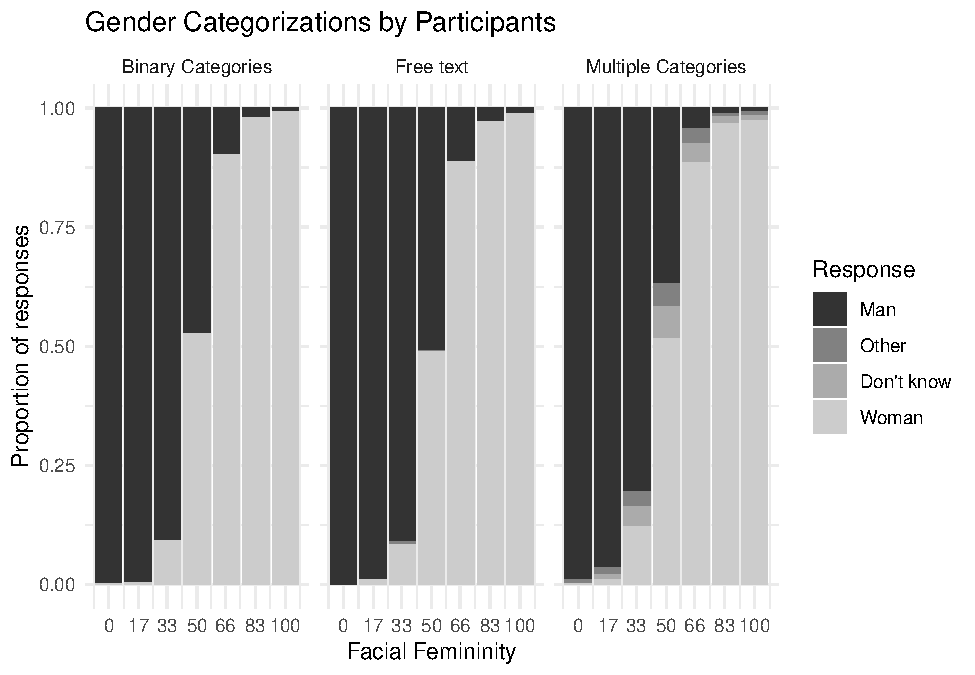
\includegraphics{resp_opts_manus23022_files/figure-latex/descriptives-1.pdf}
\caption{\label{fig:descriptives}Gender Categorizations by Participants}
\end{figure}

\begin{table}

\caption{\label{tab:loo}Relative predictive power of models describing the outcome on the categorization task}
\centering
\begin{threeparttable}
\begin{tabular}[t]{lcccc}
\toprule
  & LOO diff & St. Error diff & LOO & St. Error LOO\\
\midrule
Interaction & 0.00 & 0.00 & -234.17 & 23.23\\
Main Effect & -2.46 & 2.71 & -236.63 & 23.07\\
Null & -18.83 & 6.02 & -253.00 & 24.51\\
\bottomrule
\end{tabular}
\begin{tablenotes}[para]
\item \textit{Note.} 
\item LOO diff refers to the difference in loo between the model and the most predictive model. The first row describes the most predictive model, which is why the difference is 0
\end{tablenotes}
\end{threeparttable}
\end{table}

To investigate whether response options affected gender categorization we fit a Null Model, a Main Effects Model and an interaction model to the data. As stated, for these analyses, the Binary Categories condition was excluded, as participant did not have the option to categorize beyond the binary. The results of model comparison are presented in Table~\ref{tab:loo}.
Table~\ref{tab:loo} suggests that the Interaction model is the most predictive. However the absolute difference between the Interaction model and the Main effects model is small and importantly, the difference is small in relation to the standard error of the difference. This suggests that the data is inconclusive about which model is most suitable, although both are superior to the Null model. As model comparison did not conclusively preclude the Interaction model, we continued by testing specific, relevant contrasts using the Interaction model (see the Supplementary material for specific contrast weights).

\begin{figure}
\centering
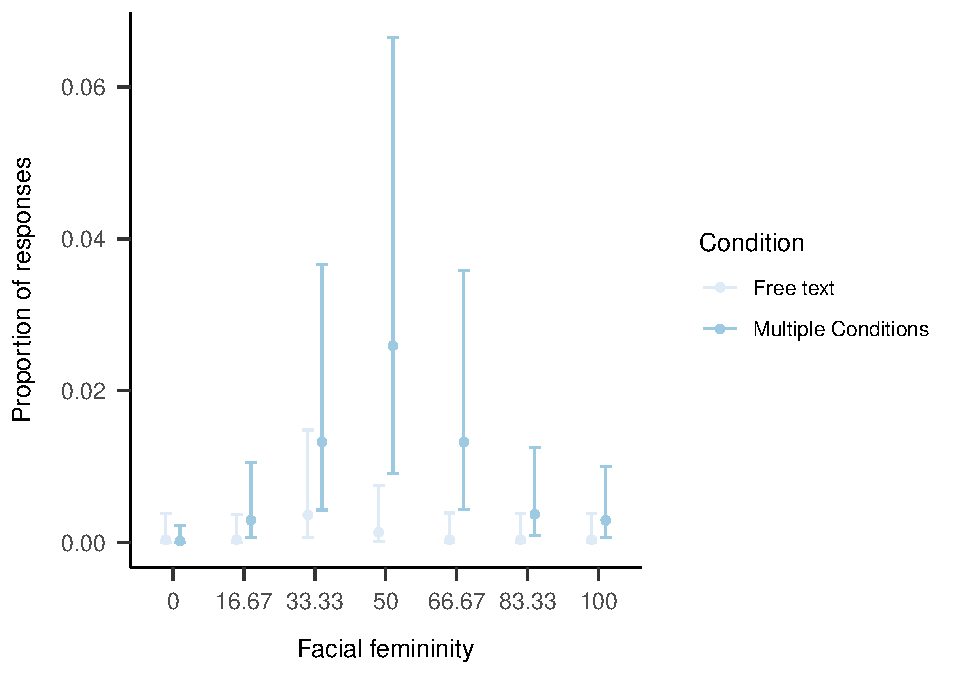
\includegraphics{resp_opts_manus23022_files/figure-latex/exp-one-inf-1.pdf}
\caption{\label{fig:exp-one-inf}Proportion of beyond-binary responses in the Multiple Categories and Free Text conditions}
\end{figure}

Model parameters are visualized in Figure~\ref{fig:exp-one-inf}. First, whether participants overall made more beyond-binary categorizations in the multiple categories condition than in the free text condition. Although the incidence was rare in both conditions (as is clear from Figure~\ref{fig:descriptives}) the evidence suggests fairly convincingly that participants made more beyond-binary categorizations in the Multiple Categories than in the Free Text is the case (OR = 59.74, CI ={[}4.71, 854.06{]}, BF\textsubscript{10}= 97.67). Additionally, based on visual inspection of Figure~\ref{fig:exp-one-inf}, which suggested that the difference between the condition was concentrated at morphs containing equal levels of femininity and masculinity (i.e.~facial femininity = 50\%), we explored whether the evidence supported this difference at facial femininity = 50\%. There was moderate evidence that participants made more beyond-binary categorizations in the Multiple Categories condition than the Free text condition at facial femininity = 50\% (OR = 61.56, CI ={[}3.90, 1,619.71{]}, BF\textsubscript{10}= 17). Lastly, we tested the difference using quadratic weights, though here the difference was inconclusive (OR = 1.22, CI = {[}0.63,2.27{]}, BF\textsubscript{10}= 0.52).

Overall the evidence suggests at least somewhat strongly that when participants have the option of using beyond-binary response options, they use them.

Subsequently, we tested whether the inclusion of non-binary response options skewed the distribution of categorization of faces as women and men. For this analysis, therefore, we tested the outcome variable \emph{binary categorization}, excluding ``other'' ``I don't know'' and any other respones in the free text.

\begin{table}

\caption{\label{tab:rq2-table}Relative predictive power of models describing the outcome on the categorization task}
\centering
\begin{threeparttable}
\begin{tabular}[t]{llccc}
\toprule
  & LOO difference & St. Error diff & LOO & St. Error LOO\\
\midrule
Main Effect & 0.00 & 0.00 & -1345.56 & 43.17\\
Null & -3.51 & 4.90 & -1349.07 & 44.12\\
Interaction & -4.84 & 3.09 & -1350.40 & 43.48\\
\bottomrule
\end{tabular}
\begin{tablenotes}[para]
\item \textit{Note.} 
\item LOO diff refers to the difference in loo between the model and the most predictive model. The first row describes the most predictive model, which is why the difference is 0
\end{tablenotes}
\end{threeparttable}
\end{table}

To test this research question, we first carried out model comparison. The results of this are presented in Table~\ref{tab:rq2-table}. Again, we compared a Null model, a Main Effects model and an Interaction model. Although the Interaction model was the worst in terms of LOO-CV, the standard errors were quite large relative to the difference, again suggesting that the model comparison was inconclusive and the existence of an interaction could not be excluded. For completeness we therefore carried out the contrast analyses using the Interaction model.

Based on the pattern in Figure~\ref{fig:descriptives}, which seems to show that in the Multiple Categories condition, participants made fewer ``man'' responses compared to the other condition, we compared the distribution of woman/man responses at facial femininity = 50\%. The evidence were slightly in favor of there being no difference between the multiple categories and the free text conditions (OR = 0.61, CI ={[}0.29, 1.28{]}, BF\textsubscript{01}= 4.80) and moderately in favor of no difference between multiple categories and binary categories conditions (OR = 0.76, CI ={[}0.37, 1.57{]}, BF\textsubscript{01}= 9.10). In other words, the evidence suggests that when participants categories faces beyond the binary, this does not skew the categorizations of women and men in any direction.

\hypertarget{discussion}{%
\section{Discussion}\label{discussion}}

Eexperiment 1 indicated that participants categorize beyond the binary when response options include more options than women and men only. However, the free text option did not differ from the binary option. Thus, the written out choices seem to act as reminders to participants. Furthermore, categorization beyond the binary affected former man and women responses to similar degrees, meaning that the ratio of women and men were still about 50/50. This did not systematically affect their overall pattern of responses in terms of woman and man categorizations.

\hypertarget{study-2}{%
\section{Study 2}\label{study-2}}

Study 2 tested whether continuous scales that measure woman and men separately reduce categorical perception. To that end, we once again borrowed from the literature on self-categorization, this time using (Bem, 1974) method of measuring gender on two separate scales.
If categorical perception occurs, ratings of woman and man should be skewed near facial femininity = 50. In other words, a face with 33.33\% facial femininity would be rated as less woman than that. Therefore, we examined the differences between the two conditions at facial femininity = 33.33\% and 66.67\%,

\hypertarget{method-1}{%
\section{Method}\label{method-1}}

\hypertarget{participants-1}{%
\subsubsection{Participants}\label{participants-1}}

Participants (\emph{N} = 49) were recruited through advertising online and on the university campus (\emph{M}\textsubscript{age}= 36.67, \emph{SD}\textsubscript{age} = 12.54).Self-identified gender was measured using an open-ended text box; 25 women and 24 men participated. Participants were monetarily compensated for their time. All participants were informed that participation was voluntary and gave written consent to participate in the study in accordance with ethical recommendations. The participants were randomly allocated to conditions.

\hypertarget{stimuli-procedure}{%
\subsection{Stimuli \& Procedure}\label{stimuli-procedure}}

The stimuli and procedure for study 2 were identical to experiment 1 but included only two conditions. Study 2 differed only the response options conditions, such that response option conditions consisted of a single dimension, which ranged from ``woman'' to ``man'' and ``multiple dimension'' which ranged from ``not woman'' to ``woman'' and ``not man'' to ``man''. For the multiple dimensions condition, participants rated the same faces according to both scales, but on separate trials. This differed from Bem (1974), who used scales of ``femininity'' and ``masculinity''. The present anchors were chosen because gender categorization was the focus of the present study.

\hypertarget{data-analysis-1}{%
\subsection{Data analysis}\label{data-analysis-1}}

Research question 3 asked whether whether participants would view faces less categorically in when they categorized them using multiple dimensions (i.e.~Not woman - Woman/Not man -Man) than when they used the single dimension (Woman-Man). We expected to see a difference between the two conditions at fecial feminiity = 33.33 and 66.67 as these were the closes to the midway point. In other words, if categorical perception is reduced, we would expect to see an interaction between condition and facial femininity level, but not a main effect. To test this, we fit a single Bayesian mixed-effects model which calculated unique fixed intercepts at each intersection of facial femininity and condition as well as varying intercepts for participants and faces (See supplemental material for full model specification). Using Savage-Dickey density ratios, we calculated the Bayes Factors for the contrasts between single dimension condition and multiple dimension at Facial Femininity = 33.37 and 66.66.

\hypertarget{results-1}{%
\section{Results}\label{results-1}}

The mean ratings in both conditions are presented in Figure~\ref{fig:descriptives-two}.

\begin{figure}
\centering
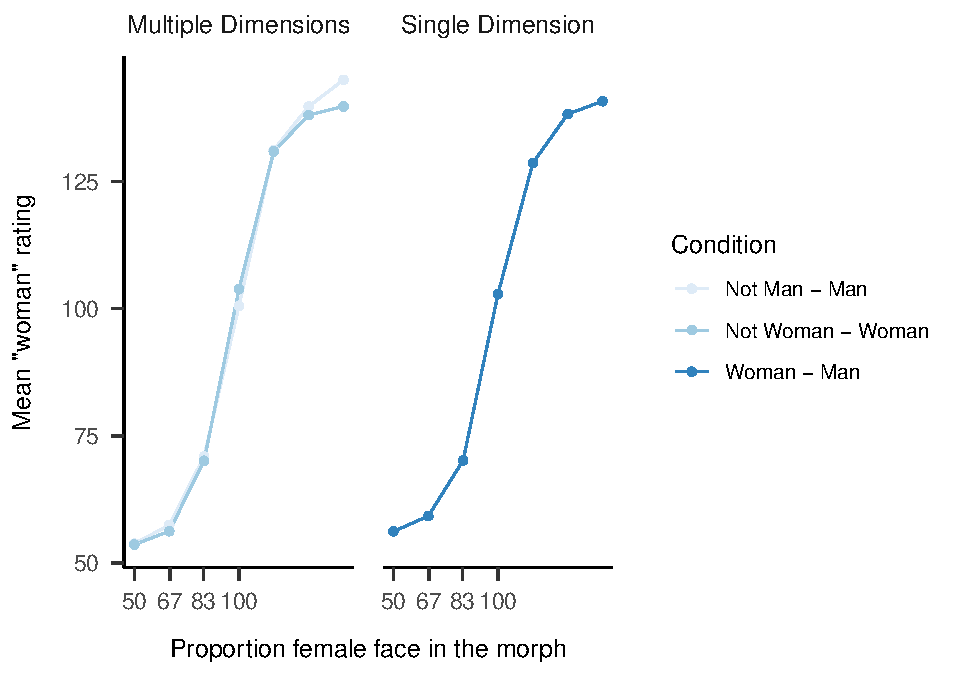
\includegraphics{resp_opts_manus23022_files/figure-latex/descriptives-two-1.pdf}
\caption{\label{fig:descriptives-two}Mean ratings of faces in Single dimension and multiple dimensions}
\end{figure}

\begin{figure}
\centering
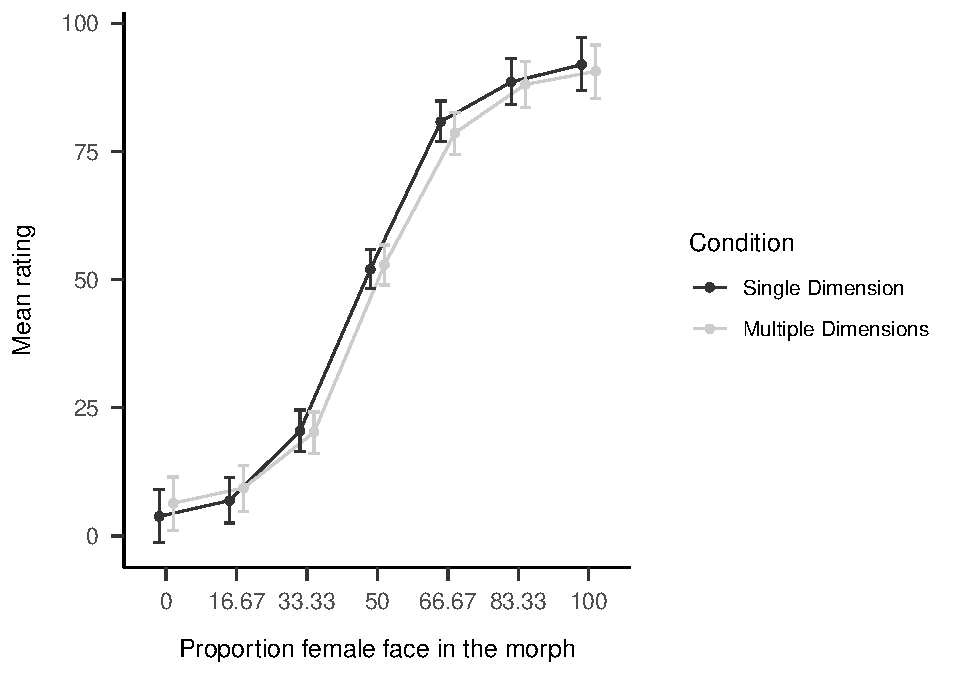
\includegraphics{resp_opts_manus23022_files/figure-latex/exp-two-inf-1.pdf}
\caption{\label{fig:exp-two-inf}Mean gender ratings in Single Dimension and Multiple Dimensions conditions}
\end{figure}

We compared the mean rating at facial femininity = 33.33 and 66.67 morph for both conditions. At facial femininity = 33.33 the evidence strongly suggested that the two conditions were the same
(Estimate = 0.28, CI ={[}-3.91, 4.51{]}, BF\textsubscript{01}= 32.28). This was also the case at facial femininity = 66.67
(Estimate = 2.29, CI ={[}-2.03, 6.57{]}, BF\textsubscript{01}= 18.97). Overall, both conditions showed fairly strong tendencies toward categorical perception and they did not differ in this regard.

\hypertarget{discussion-1}{%
\section{Discussion}\label{discussion-1}}

Study 2 showed that participants exhibited signs of categorical perception when rating faces in terms of gender. Additionally, this did not depend on response option condition; response options which did not present women and men as opposing categories led to an equal amount of categorical perception as response options that did. Indeed a highly binary view of gender was present and participants treated womanhood and manhood as opposites even the scale would allow them to be more flexible.

\hypertarget{general-discussion}{%
\section{General discussion}\label{general-discussion}}

In two experiments, we tested how response options in gender categorization of others influence binary gender categorization. Specifically, the results provided strong evidence that participants only use beyond-binary options to categorize faces when such options are provided explicitly. Free text answers or continuous scales did not affect participants binary gender categorization. Additionally, response options which did not present women and men as opposing categories did not induce participant's perception of gender in faces to be less binary.

These findings are somewhat consistent with previous research, such as the work of Saperstein and Westbrook (2021) and Lindqvist et al. (2020), which has shown that including flexible response options allow participants to better express themselves. Unlike the literature on self-categorization, increased freedom did not increase the gender diversity of participants' categorizations, rather explicit reminders seem to have the largest effect. When participants categorized women or men on continuous scales, the results differ from Bem (1974) who found that participants categorize their own femininity and masculinity independently of each other. Rather, when categorizing others, the participants in the present study seemed to treat women and men as opposites, even when the response options did not pose them as such. Both of these deviations from the previous literature likely stem from the substantial difference between indicating one's own gender and categorizing that of others.

It is worth noting that this study only examined participants' stated categorizations, and it is possible that they may have made other categorizations internally that were not reflected in their responses. However, it is important to recognize that a purely behavioral study such as this cannot fully capture the neurological processes underlying gender perception, which may require more sophisticated techniques such as fMRI and EEG (Kloth et al., 2010; Stolier \& Freeman, 2017).

In this study we aggregated responses that did not indicate woman or man. In the multiple response option condition, both ``I don't know'' and ``Non-binary'' were included as a beyond binary categorization. We justified this on the basis that what we were interested in is any categorization beyond the binary. However, these two options are not the same. Furthermore, it is important to note that no matter how a person looks, it is impossible to know their binary or non-binary gender identity (Richards et al., 2016). Therefore, if a person aims to be inclusive and not categorize in a binary way, then abstaining from categorizing, for examle by selecting ``I don't know'' is always the best option.

In the introduction we raised the possibility that findings within gender categorization research may be biased from a sole reliance on binary response options. Based on the present results, this seems unlikely. Instead, it seems that the societal norm to treat gender as binary is the strongest determinant participants gender categorizations. Even so, we recommend researchers to carefully consider their measurements of gender categorization. Open text-boxes, forced choice-alternatives and dimensional scales are all viable alternatives. Even researchers who are primarily interested in binary categorizations should consider including beyond-binary alternatives, to avoid perpetuating the binary gender norm and to accurately represent the diversity of gender.

\hypertarget{conclusion}{%
\paragraph{Conclusion}\label{conclusion}}

In two experiments we tested how different response alternatives affected gender categorizations. Participants were more likely to categorize faces beyond the binary when using a forced-choice paradigm including ``non-binary'' and ``I don't know'' than when using a free text option, or slider scales. In comparison to self-identification questions where open ended responses are seen as the most inclusive alternative (Lindqvist et al., 2020), categorization of others benefit from response options that explicitly reminds participants that not all people identify as women or men.

\newpage

\hypertarget{references}{%
\section{References}\label{references}}

\hypertarget{refs}{}
\begin{CSLReferences}{1}{0}
\leavevmode\vadjust pre{\hypertarget{ref-ansara_methodologies_2014}{}}%
Ansara, Y. G., \& Hegarty, P. (2014). Methodologies of misgendering: Recommendations for reducing cisgenderism in psychological research. \emph{Feminism \& Psychology}, \emph{24}(2), 259--270. \url{https://doi.org/10.1177/0959353514526217}

\leavevmode\vadjust pre{\hypertarget{ref-R-papaja}{}}%
Aust, F., \& Barth, M. (2022). \emph{{papaja}: {Prepare} reproducible {APA} journal articles with {R Markdown}}. \url{https://github.com/crsh/papaja}

\leavevmode\vadjust pre{\hypertarget{ref-bem_measurement_1974}{}}%
Bem, S. L. (1974). \emph{{THE} {MEASUREMENT} {OF} {PSYCHOLOGICAL} {ANDROGYNY}}. 8.

\leavevmode\vadjust pre{\hypertarget{ref-R-brms_a}{}}%
Bürkner, P.-C. (2017). {brms}: An {R} package for {Bayesian} multilevel models using {Stan}. \emph{Journal of Statistical Software}, \emph{80}(1), 1--28. \url{https://doi.org/10.18637/jss.v080.i01}

\leavevmode\vadjust pre{\hypertarget{ref-R-brms_b}{}}%
Bürkner, P.-C. (2018). Advanced {Bayesian} multilevel modeling with the {R} package {brms}. \emph{The R Journal}, \emph{10}(1), 395--411. \url{https://doi.org/10.32614/RJ-2018-017}

\leavevmode\vadjust pre{\hypertarget{ref-R-brms_c}{}}%
Bürkner, P.-C. (2021). Bayesian item response modeling in {R} with {brms} and {Stan}. \emph{Journal of Statistical Software}, \emph{100}(5), 1--54. \url{https://doi.org/10.18637/jss.v100.i05}

\leavevmode\vadjust pre{\hypertarget{ref-campanella_categorical_2001}{}}%
Campanella, S., Chrysochoos, A., \& Bruyer, R. (2001). Categorical perception of facial gender information: Behavioural evidence and the face-space metaphor. \emph{Visual Cognition}, \emph{8}(2), 237--262. \url{https://doi.org/10.1080/13506280042000072}

\leavevmode\vadjust pre{\hypertarget{ref-carleton_assessing_2022}{}}%
Carleton, R. N., McCarron, M., Krätzig, G. P., Sauer-Zavala, S., Neary, J. P., Lix, L. M., Fletcher, A. J., Camp, R. D., Shields, R. E., Jamshidi, L., Nisbet, J., Maguire, K. Q., MacPhee, R. S., Afifi, T. O., Jones, N. A., Martin, R. R., Sareen, J., Brunet, A., Beshai, S., \ldots{} Asmundson, G. J. G. (2022). Assessing the impact of the royal canadian mounted police ({RCMP}) protocol and emotional resilience skills training ({ERST}) among diverse public safety personnel. \emph{{BMC} Psychology}, \emph{10}(1), 295. \url{https://doi.org/10.1186/s40359-022-00989-0}

\leavevmode\vadjust pre{\hypertarget{ref-cloutier_perceptual_2005}{}}%
Cloutier, J., Mason, M. F., \& Macrae, C. N. (2005). The perceptual determinants of person construal: Reopening the social-cognitive toolbox. \emph{Journal of Personality and Social Psychology}, \emph{88}(6), 885--894. \url{https://doi.org/10.1037/0022-3514.88.6.885}

\leavevmode\vadjust pre{\hypertarget{ref-cronin_younger_2022}{}}%
Cronin, K. A., Leahy, M., Ross, S. R., Wilder Schook, M., Ferrie, G. M., \& Alba, A. C. (2022). Younger generations are more interested than older generations in having non-domesticated animals as pets. \emph{{PLOS} {ONE}}, \emph{17}(1), e0262208. \url{https://doi.org/10.1371/journal.pone.0262208}

\leavevmode\vadjust pre{\hypertarget{ref-dagostino_organizational_2022}{}}%
D'Agostino, M., Levine, H., Sabharwal, M., \& Johnson-Manning, A. C. (2022). Organizational practices and second-generation gender bias: A qualitative inquiry into the career progression of u.s. State-level managers. \emph{The American Review of Public Administration}, \emph{52}(5), 335--350. \url{https://doi.org/10.1177/02750740221086605}

\leavevmode\vadjust pre{\hypertarget{ref-dascenzo_imagining_2014}{}}%
D'Ascenzo, S., Tommasi, L., \& Laeng, B. (2014). Imagining sex and adapting to it: Different aftereffects after perceiving versus imagining faces. \emph{Vision Research}, \emph{96}, 45--52. \url{https://doi.org/10.1016/j.visres.2014.01.002}

\leavevmode\vadjust pre{\hypertarget{ref-debruine_webmorph_2018}{}}%
DeBruine, L. (2018). \emph{{WebMorph}. {WebMorph}}. \url{https://webmorph.org/}

\leavevmode\vadjust pre{\hypertarget{ref-debruine_face_2017}{}}%
DeBruine, L. M., \& Jones, B. C. (2017). Face research lab london set. \emph{Figshare}. \url{https://doi.org/10.6084/m9.figshare.5047666}

\leavevmode\vadjust pre{\hypertarget{ref-gottgens_impact_2022}{}}%
Göttgens, I., Darweesh, S. K. L., Bloem, B. R., \& Oertelt-Prigione, S. (2022). The impact of multiple gender dimensions on health-related quality of life in persons with parkinson's disease: An exploratory study. \emph{Journal of Neurology}, \emph{269}(11), 5963--5972. \url{https://doi.org/10.1007/s00415-022-11228-2}

\leavevmode\vadjust pre{\hypertarget{ref-habibi_spontaneous_2012}{}}%
Habibi, R., \& Khurana, B. (2012). Spontaneous gender categorization in masking and priming studies: Key for distinguishing jane from john doe but not madonna from sinatra. \emph{{PLoS} {ONE}}, \emph{7}(2), e32377. \url{https://doi.org/10.1371/journal.pone.0032377}

\leavevmode\vadjust pre{\hypertarget{ref-hyde_future_2018}{}}%
Hyde, J. S., Bigler, R. S., Joel, D., Tate, C. C., \& Anders, S. M. van. (2018). The future of sex and gender in psychology: Five challenges to the gender binary. \emph{American Psychologist}. \url{https://doi.org/10.1037/amp0000307}

\leavevmode\vadjust pre{\hypertarget{ref-jung_automaticity_2019}{}}%
Jung, K. H., White, K. R. G., \& Powanda, S. J. (2019). Automaticity of gender categorization: A test of the efficiency feature. \emph{Social Cognition}, \emph{37}(2), 122--144. \url{https://doi.org/10.1521/soco.2019.37.2.122}

\leavevmode\vadjust pre{\hypertarget{ref-kloth_neural_2010}{}}%
Kloth, N., Schweinberger, S. R., \& Kovács, G. (2010). Neural correlates of generic versus gender-specific face adaptation. \emph{Journal of Cognitive Neuroscience}, \emph{22}(10), 2345--2356. \url{https://doi.org/10.1162/jocn.2009.21329}

\leavevmode\vadjust pre{\hypertarget{ref-kurz_doing_2023}{}}%
Kurz, S. (2023). \emph{Doing bayesian data analysis in brms and the tidyverse}. \url{https://bookdown.org/content/3686/}

\leavevmode\vadjust pre{\hypertarget{ref-lindqvist_what_2020}{}}%
Lindqvist, A., Sendén, M. G., \& Renström, E. A. (2020). What is gender, anyway: A review of the options for operationalising gender. \emph{Psychology \& Sexuality}, 1--13. \url{https://doi.org/10.1080/19419899.2020.1729844}

\leavevmode\vadjust pre{\hypertarget{ref-ma_chicago_2015}{}}%
Ma, D. S., Correll, J., \& Wittenbrink, B. (2015). The chicago face database: A free stimulus set of faces and norming data. \emph{Behavior Research Methods}, \emph{47}(4), 1122--1135. \url{https://doi.org/10.3758/s13428-014-0532-5}

\leavevmode\vadjust pre{\hypertarget{ref-mogilski_relative_2018}{}}%
Mogilski, J. K., \& Welling, L. L. M. (2018). The relative contribution of jawbone and cheekbone prominence, eyebrow thickness, eye size, and face length to evaluations of facial masculinity and attractiveness: A conjoint data-driven approach. \emph{Frontiers in Psychology}, \emph{9}, 2428. \url{https://doi.org/10.3389/fpsyg.2018.02428}

\leavevmode\vadjust pre{\hypertarget{ref-R-base}{}}%
R Core Team. (2022). \emph{R: A language and environment for statistical computing}. R Foundation for Statistical Computing. \url{https://www.R-project.org/}

\leavevmode\vadjust pre{\hypertarget{ref-richards_non-binary_2016}{}}%
Richards, C., Bouman, W. P., Seal, L., Barker, M. J., Nieder, T. O., \& T'Sjoen, G. (2016). Non-binary or genderqueer genders. \emph{Int Rev Psychiatry .}, \emph{28(1)}, 95--102.

\leavevmode\vadjust pre{\hypertarget{ref-saperstein_categorical_2021}{}}%
Saperstein, A., \& Westbrook, L. (2021). Categorical and gradational: Alternative survey measures of sex and gender. \emph{European Journal of Politics and Gender}, \emph{4}(1), 11--30. \url{https://doi.org/10.1332/251510820X15995647280686}

\leavevmode\vadjust pre{\hypertarget{ref-stolier_neural_2017}{}}%
Stolier, R. M., \& Freeman, J. B. (2017). A neural mechanism of social categorization. \emph{The Journal of Neuroscience}, \emph{37}(23), 5711--5721. \url{https://doi.org/10.1523/JNEUROSCI.3334-16.2017}

\leavevmode\vadjust pre{\hypertarget{ref-webster_adaptation_2004}{}}%
Webster, M. A., Kaping, D., Mizokami, Y., \& Duhamel, P. (2004). Adaptation to natural facial categories. \emph{Nature}, \emph{428}(6982), 557--561. \url{https://doi.org/10.1038/nature02420}

\leavevmode\vadjust pre{\hypertarget{ref-R-tidyverse}{}}%
Wickham, H., Averick, M., Bryan, J., Chang, W., McGowan, L. D., François, R., Grolemund, G., Hayes, A., Henry, L., Hester, J., Kuhn, M., Pedersen, T. L., Miller, E., Bache, S. M., Müller, K., Ooms, J., Robinson, D., Seidel, D. P., Spinu, V., \ldots{} Yutani, H. (2019). Welcome to the {tidyverse}. \emph{Journal of Open Source Software}, \emph{4}(43), 1686. \url{https://doi.org/10.21105/joss.01686}

\leavevmode\vadjust pre{\hypertarget{ref-wittlin_about_2018}{}}%
Wittlin, N. M., Dovidio, J. F., LaFrance, M., \& Burke, S. E. (2018). About face: Memory for transgender versus cisgender targets' facial appearance. \emph{Journal of Experimental Social Psychology}, \emph{78}, 77--92. \url{https://doi.org/10.1016/j.jesp.2018.04.009}

\leavevmode\vadjust pre{\hypertarget{ref-zhao_own-_2008}{}}%
Zhao, L., \& Bentin, S. (2008). Own- and other-race categorization of faces by race, gender, and age. \emph{Psychonomic Bulletin \& Review}, \emph{15}(6), 1093--1099. \url{https://doi.org/10.3758/PBR.15.6.1093}

\end{CSLReferences}


\end{document}
